%%%%%%%%%%%%%%%%%%%%%%%%%%%%%%%%%%%%%%%%%%%%%%%%%%%%%%%%%%%%%%%%%%%%%%%%%%%%%%%%
%2345678901234567890123456789012345678901234567890123456789012345678901234567890
%        1         2         3         4         5         6         7         8

\documentclass[letterpaper, 10pt, conference]{ieeeconf}   % Comment this line out
                                                          % if you need a4paper
%\documentclass[a4paper, 10pt, conference]{ieeeconf}      % Use this line for a4
                                                          % paper

\IEEEoverridecommandlockouts                              % This command is only
                                                          % needed if you want to
                                                          % use the \thanks command
\overrideIEEEmargins
% See the \addtolength command later in the file to balance the column lengths
% on the last page of the document

% The following packages can be found on http:\\www.ctan.org
\usepackage{graphicx}  % for pdf, bitmapped graphics files
%\usepackage{epsfig}   % for postscript graphics files
%\usepackage{mathptmx} % assumes new font selection scheme installed
%\usepackage{times}    % assumes new font selection scheme installed
%\usepackage{amsmath}  % assumes amsmath package installed
%\usepackage{amssymb}  % assumes amsmath package installed
\usepackage{CJKutf8}   % for Chinese character support
\usepackage{setspace}  % Chinese characters need larger line height
\usepackage{hyperref}  % for citing websites in BibTeX
\usepackage{booktabs}  % for publication quality tables
\usepackage{longtable} % for multi-page tables
\usepackage{array}     % for fixed column widths

\title{\LARGE \bf
社群網站上之政治活動分析:以台灣 2016 年總統選舉為例$^{\ast}$
}

\author{\parbox{3 in}{\centering 學生:蒲郁文$^{\dagger}$}
        \hspace*{0.5 in}
        \parbox{3 in}{\centering 指導教授:孫春在 教授$^{\ddagger}$}
        \thanks{$^{\ast}$學士論文。本研究未接收任何個人及團體贊助。}
        \thanks{$^{\dagger}$國立交通大學資訊工程學系,{\tt\small ywpu@cs.nctu.edu.tw}。}
        \thanks{$^{\ddagger}$國立交通大學資訊工程學系,{\tt\small ctsun@cs.nctu.edu.tw}。}
}

\begin{document}
\begin{CJK}{UTF8}{bsmi}
\onehalfspacing
\refname{參考文獻}
\figurename{圖}
\tablename{表}
\newcolumntype{L}[1]{>{\raggedright\arraybackslash}p{#1}}
\newcolumntype{C}[1]{>{\centering\arraybackslash}p{#1}}
\newcolumntype{R}[1]{>{\raggedleft\arraybackslash}p{#1}}

\maketitle
\thispagestyle{empty}
\pagestyle{empty}

%%%%%%%%%%%%%%%%%%%%%%%%%%%%%%%%%%%%%%%%%%%%%%%%%%%%%%%%%%%%%%%%%%%%%%%%%%%%%%%%

\begin{abstract}
摘要\enskip---\enskip可以輸入繁體字了。教育雲端服務平臺將進行資安設備調整作業,並於本次作業時程完成後,%
進行網站功能測試,屆時網路服務將會中斷,造成您的不便,敬請見諒。獲得快速的翻譯。%
應該還要有一行,不可能只寫那麼少。可是這樣還不夠多,還不會換行。可以再給我多一點嗎,我很需要換下一行。%
臺灣東部地區有局部短暫陣雨,其他地區及澎湖、金門、馬祖為多雲到晴,午後中南部地區及北部山區亦有局部短暫雷陣雨。%
明日東海北部平均風力將稍減弱。本局將盡力確保其即時性及正確性。%
\end{abstract}

\begin{keywords}
關鍵字\enskip---\enskip社群媒體、自動化內容分析、社會網絡分析、數位行動主義、政治參與%
\end{keywords}

%%%%%%%%%%%%%%%%%%%%%%%%%%%%%%%%%%%%%%%%%%%%%%%%%%%%%%%%%%%%%%%%%%%%%%%%%%%%%%%%

\section*{一、緒論}

社群網站的興起不僅改變了我們的社交生活,更改變了許多國家政治與權力的運作規則。%
在國內外皆有愈來愈多政治團體與公民團體透過網路來散佈其理念;%
許多具引響力的社會運動也是透過網路來連結潛在支持者或動員大眾;%
網路工具的靈活運用甚至還成為候選人能否贏得選舉的關鍵。%

這種利用網際網路來號召群眾、表達訴求的作法被稱為數位行動主義(digital activism)。%
發生在伊朗的綠色革命(Green Movement)、北非及中東的阿拉伯之春(Arab Spring)、%
美國的佔領華爾街運動(Occupy Wall Street),皆被人們普遍認為與網際網路,特別是社群媒體,有密切的關連。%
網際網路、社群媒體對社會與政治的影響也成為許多學者關注的新焦點。%

同樣的趨勢也發生在台灣。%
從洪仲丘事件、太陽花學運到反黑箱課綱運動,網際網路均對這些社會運動的促成扮演了相當關鍵的角色。%
這也讓許多社會學家、政治學家、傳播學家與計算機科學家開始對台灣的數位行動主義熱潮產生興趣。%
這不但是一個相當新穎的、跨領域的研究主題,這方面的研究對當今台灣社會也是相當重要的。%

2016 年總統選舉競選期間,各政黨、候選人、利益團體與意見領袖皆大量使用%
臉書粉絲專頁(Facebook Pages)來與人民互動並宣揚其政治理念。%
多數民眾也相信這些網路宣傳確實有效引響了選舉的得票數。%
然而這些社群網站上的政治活動是否存在著某些機制?我們能夠利用電腦來分析這些現象嗎?還有許許多多的問題有待我們回答。%
本研究的目的便是嘗試使用資訊科技,以創新的方法分析這些使用者在臉書粉絲專頁上的公開貼文,探討使用者於社群網站上之政治活動的模式。%
由於在台灣推特(Twitter)較不盛行,人們使用的社群網站以臉書(Facebook)為主,因此本研究的重心也將放在臉書上。%

\subsection*{對數位行動主義的批判}

儘管人們普遍同意數位行動主義能有效促進民主政治,這個趨勢仍然伴隨了一些潛在的隱憂。%
常見對數位行動主義的批評包含:%
\,(1) 數位落差(digital divide):%
由於經濟、教育等差異,有些族群缺少機會接觸資訊科技,或者沒有能力使用資訊科技。%
\,(2) 民粹主義(populism):%
網路本質上便具有民粹主義、安那其(anarchy)、去中心化(decentralization)等特性,網路輿論的品質可能偏低。%
\,(3) 懶人行動主義(slacktivism):%
並沒有參與什麼實際的行動,僅是在網路上分享自己關心的社會議題,便自以為自己已經對這個議題做出了貢獻。%
\,(4) 鍵擊行動主義(clicktivism):%
類似懶人行動主義,若一味地追求點擊率、做網路行銷,可能反而會忽略了實際的行動。%
\,(5) 網路巴爾幹化(cyberbalkanization):%
由於商業壟斷、政治審查、或是個人不願意接觸與自己立場相左的訊息等因素,使網際網路逐漸分裂、解體。%

\subsection*{資訊科技與人文社會跨領域研究的挑戰與契機}

近年來,愈來愈多學者開始嘗試將計算機科學應用於人文社會科學領域,%
建立了數位典藏(digital archives)、數位人文(digital humanities)、計算社會科學(computational social science)、%
計算社會學(computational sociology)、社會模擬(social simulation)等新興研究領域。%
然而,這樣的跨領域研究是否真的有價值一直是備受爭議的。%
以下舉出一些此類研究常受到的批評,以及我從事此類研究的立場。%

常見對數位人文的批評包含:%
\,(1) 只是用一些空洞的戲法來賣弄他們的研究能力,而沒有真正做出什麼新的分析。%
\,(2) 容易忽略種族、階級、性別、文化、意識型態等面向。%
\,(3) 在這個一切都已經被商品化了的現代社會中,人文學科日漸式微。但數位人文卻頂著科技的光環,而獲得了相當高的經費與聲望。%
\,(4) 研究者的背景不夠多元,其研究可能帶有某些偏見。%

常見對社會模擬的批評包含:%
\,(1) 將現實社會過度地簡化為一般化的法則。%
\,(2) 模擬的成果仰賴預先建立好的模型,難以發現新的法則。%
\,(3) 預先建立的模型往往充滿偏見。%
\,(4) 模擬的成果並不能反映出現實社會的情況。%

我的回應是,我認為傳統社會科學研究法仍是不可或缺的:%
\,(1) 並非所有問題都適合使用電腦來分析或模擬,有些現象無法被量化或歸納出一般化的法則。%
\,(2) 人文社會科學做的不只是資料分析、統計而已,還包含人文關懷、詮釋、思辨、批判等。%
\,(3) 因此田野工作、民族誌、訪談等研究法仍有其彌足珍貴的價值。%

然而資訊科技仍然能對人文學科做出貢獻:%
\,(1) 數位人文提供了一個全新的視野來探究傳統上屬於人文社會科學領域的問題。%
\,(2) 資訊科技能幫助人文學者更有效率地獲得知識。%
\,(3) 資料探勘(data mining)、自然語言處理(natural language processing)等技術使一些過去被認為窒礙難行的研究成為可能。%

\section*{二、文獻探討}

過去已有多位學者考察了社群網站在競選活動中的使用,%
例如 Larsson and Moe (2012) 研究了 2010 年瑞典選舉競選期間推特的使用。\cite{c1} %
該研究的作法是,蒐集競選期間含有特定 hashtag 的推文,進行社會網絡分析(social network analysis)。%

該研究做了以下分析:%
\,(1) 不同時間推文數量的變化。%
\,(2) 各種推文類型(一般、提及、轉推)所佔的比例。%
\,(3) 列出最活躍的使用者及其推文數量,並調查其身份背景。%
\,(4) 活躍用戶的「提及」網絡圖(透過資料視覺化)。%
\,(5) 呈上,將使用者分為發送者、接受者、兩者皆是,並調查其身份背景。%
\,(6) 活躍用戶的「轉推」網絡圖(透過資料視覺化)。%
\,(7) 呈上,將使用者分為轉推者、被轉推者、兩者皆是,並調查其身份背景。%

該研究發現:%
\,(1) 推文數量的變化反應了線下競選活動的情勢。%
\,(2) 大部份的推文都是由少部份的活躍用戶所發出。%
\,(3) 大部份的活躍用戶都是政治菁英,然而,平民的聲音仍具有一定的影響力。%
\,(4) 大部份的推文都是一般推文,然而,許多活躍用戶仍會在推特上與人討論。%

然而該研究也具有以下限制:%
\,(1) 只有極少數的民眾有使用推特。%
\,(2) 只蒐集含有特定 hashtag 的推文。%
\,(3) 應分析不同情境下的使用情形,加以比較。%
另外,該研究也讓我想到一個值得進一步探究的問題,那就是,如何區別真人用戶與機器用戶?%

另外 Zhang et al. (2010) 則研究了社群網站對公民的政治態度與行為的引響。\cite{c2} %
該研究參考了以下既有理論:%
\,(1) 社會資本(social capital)、大眾媒體(mass media)、人際討論(interpersonal discussion)、%
社群網站(social networking sites)都會影響公民參與(civic participation)和政治參與(political participation)。%
\,(2) 影響個人的政治態度與行為的因子有:政治興趣(political interest)、政治效能(political efficacy)、%
政治信任(political trust)、政黨認同(party identification)。%

該研究的作法是採用電話調查,%
應變數(dependent variable)為政治參與、公民參與、對政府的信任,%
自變數(independent variable)為社群網站之依賴、政治之人際討論,%
控制變數(control variable)為政治效能、意識形態、政治興趣、年齡、性別、種族、教育程度。%
最後,進行階層式迴歸分析(hierarchical regression analysis)。%

該研究發現:%
\,(1) 社群網站的使用與公民參與的提升呈現顯著的正相關,與政治參與、對政府的信任則無明顯關聯。%
\,(2) 討論政治議題有助於促進公民參與和政治參與,無助於提升對政府的信任。%
\,(3) 教育程度愈高,愈有可能參與公民活動和政治活動,但對政府的信任卻愈低。%
\,(4) 然而,政治效能感較高者,其政治信任感也較高。%

然而該研究也具有以下限制:%
\,(1) 樣本可能不夠具代表性,有超過四分之三的受訪者都完全不依賴社群網站。%
\,(2) 除了公民參與/政治參與的二分法外,是否還有更適當的分類法?%
另外,該研究也讓我想到兩個值得進一步探究的問題:%
\,(1) 調查結果顯示社群網站的使用無助於促進政治參與,這項發現在東方國家也成立嗎?%
\,(2) 調查結果顯示年長者較積極參與政治活動,當今台灣社會也是如此嗎?%

最後 Hosch-Dayican et al. (2016) 則研究了 2012 年德國議會選舉競選期間公民如何在推特上遊說他人。\cite{c3} %
其研究方法為:%
\,(1) 資料蒐集(data collection):%
先選定數個 hashtag,再透過滾雪球抽樣(snowball sampling),找出其他相關的 hashtag。%
蒐集選舉期間含有這些 hashtag 的推文。%
\,(2) 資料清理(data cleaning):%
接著,需刪去誤判的推文。%
先刪去語言與地區皆不符的推文,再從剩下的推文中篩選出直接與選舉有關的推文。%
\,(3) 操作化(operationalization):%
承上,先將推文分為「競選活動」與「非競選活動」兩種類型,再將屬於「競選活動」的推文分為%
「說服型競選(persuasive campaigning)」與「攻擊型競選(negative campaigning)」兩種類型。%
\,(4) 自動化內容分析(automated content analysis):%
以上篩選與分類的過程仰賴質化內容分析(qualitative content analysis)。%
採用監督式學習(supervised learning),先由研究者做一小部份的樣本,再用它來訓練機器。%
具體作法包含克氏 α 係數(Krippendorff's alpha)、單純貝氏分類器(naive Bayes classifier)、%
一元語法(unigram)與二元語法(bigram)、詞幹提取(stemming)、十等分交叉驗證%
(10-fold cross-validation)等等。%

該研究做了以下分析:%
\,(1) 各種推文類型(非競選活動、說服型競選、攻擊型競選)與各種用戶類型(政黨/政治人物、媒體/記者、平民)%
的組合的推文所佔的比例。%
\,(2) 從屬於「競選活動」的推文中隨機抽樣,進行更深入的內容分析。%
不論是「說服型競選」還是「攻擊型競選」,其推文皆可分為直接宣傳(明確表態要/不要投給誰)%
與間接宣傳(僅表達支持/反對意見)兩種。%

該研究發現:%
\,(1) 平民相當投入線上政治活動。%
\,(2) 政黨/政治人物最常採取說服型競選,媒體/記者及平民最常發佈非競選活動的推文。%
\,(3) 相較於其他用戶類型,平民採取攻擊型競選的比例最高。%
儘管在所有的用戶類型中,用戶採取攻擊型競選的比例都是最低的。%
\,(4) 說服型競選相當程度地採用「轉推」的形式。%
直接宣傳的部份,常出現含有投票動機或投票行為的貼文,尤其是在選舉前夕和選舉當天。%
間接宣傳的部份,常出現對新聞報導、採訪、辯論的回應。%
\,(5) 攻擊型競選則多為間接宣傳,採用「轉推」的形式,引用政黨/政治人物的推文。%
比起政治菁英,平民的推文更包含了對採訪與辯論的回應,以及對政黨/政治人物的不滿與憤怒。%
\,(6) 平民被歸類為攻擊型競選的推文大部份都是在宣洩情緒與意見,而不是以進行攻擊型競選為目的。%

該文作者建議後續研究者,進一步分析「轉推」網絡,並探討線上競選的後果。%
另外,該研究也讓我想到幾個值得進一步探究的問題:%
\,(1) 這份研究只有區別政治菁英與平民,忽略了使用者間的其他差異(例如社會經濟背景)。%
\,(2) 採用監督式學習能降低解讀反諷文章的錯誤率到什麼程度?%
\,(3) 台灣的使用者是否也具有如此高的素養,僅將近 20\% 的網路貼文被歸類為攻擊型競選?%

\section*{三、研究問題與方法}

本研究分析的資料來自 2016 年台灣總統選舉競選期間臉書各大政治性粉絲專頁之公開資料。%
本研究進行的分析包含以下四個部份:%
\begin{itemize}
\item 貼文數量對時間的關係圖。\\
各政黨/侯選人/意見領袖的貼文數量。%
\item 每個時間區間最熱門的關鍵字分別是哪些?\\
嘗試透過關鍵字分析,\\
找出各政黨/侯選人/意見領袖最重視的議題。%
\item 有多少比例的貼文是攻擊型競選?\\
哪些政黨/候選人/意見領袖、什麼時候\\
最常使用攻擊型競選?%
\item 各發文者與其分享的貼文的來源之網絡圖。\\
特定族群是否會傾向於分享特定來源的資訊?%
\end{itemize}

本研究主要採用量化研究(quantitative research),著重於資料分析。%
在研究方法上,本研究結合了多種現代計算機科學理論與技術:%
\begin{itemize}
\item 資料探勘(data mining)%
\item 機器學習(machine learning)%
\item 自然語言處理(natural language processing)%
\item 資料視覺化(data visualization)%
\end{itemize}

本研究具體的研究步驟如下所述。%

\subsection*{資料蒐集(data collection)}

使用 Facebook Graph API 蒐集競選期間(投票日前三個月至投票日止)台灣各大政治性粉絲專頁之公開資料。%
本研究蒐集的資料以貼文為主,同時亦包含一些附屬的詮釋資料(metadata),例如發文時間、分享的連結等。%
為保護個人隱私,本研究只蒐集粉絲專頁上的公開資料,不蒐集任何個別使用者的資料。%

採用何種方法決定欲蒐集的粉絲專頁清單,對研究結果有極大的引響。%
為確保本研究的中立性,我參考 Socialbakers \cite{c4} 及 Likeboy \cite{c5} 提供之社群媒體統計數據,%
輔以我個人的自身經驗,整理出一份台灣熱門政治性粉絲專頁的清單。%
得到粉絲專頁清單後,我還做了進一步的篩選。%
我查詢這些粉絲專頁最新的按讚數,將它們依按讚數由高到低排序。%
擁有超過一萬個讚的粉絲專頁共計有 135 個,這些粉絲專頁便是我最終選定的蒐集對象。%

完成後,本研究共取得了 18,967 筆臉書貼文,來自 135 個台灣熱門的政治性粉絲專頁。%

\subsection*{斷詞(word segmentation)}

下個步驟是進行文本斷詞,也就是將一篇文章拆解成一個個的單詞。%
例如「維根斯坦是二十世紀最有影響力的哲學家之一。」這句話可以被拆解成%
「維根斯坦」、「是」、「二十世紀」、「最」、「有」、「影響力」、「的」、「哲學家」、「之一」、「。」等單詞。%
斷詞是自然語言處理中最基本的步驟,文本必需先經過斷詞處理,才得以進一步分析。%

本研究採用中央研究院資訊科學研究所中文詞知識庫小組所研發之中文斷詞系統 \cite{c6},%
搭配我自行開發之中文斷詞系統 Python 客戶端程式 \cite{c7},為蒐集到的貼文進行斷詞。%
本研究之所以選擇中央研究院的中文斷詞系統,是因為此系統正確率高(其研發團隊亦稱此系統之正確率約為 95\% $\sim$ 96\%),%
且相較於其他非台灣開發的中文斷詞系統,此系統對台灣本地的文本有較好的表現。%
若要採用其他斷詞系統,可能得用台灣本地的語料重新訓練,才能達到同樣的表現。%
另外,良好的未知詞辨識能力也是此系統的一大優點。%

由於本研究分析的文本是社群網站上的貼文,其形式較不嚴謹,%
常有錯別字、文法錯誤、使用空格或換行代替逗號或句號、夾雜表情符號或特殊字元等情形,%
故我在每則貼文開始斷詞前均會先對貼文進行簡單的預處理(pre-processing)。%
斷詞全部完成後,我更做了完整性測試(integrity test),檢查斷詞前與斷詞後的貼文是否一致。%
測試結果顯示斷詞系統相當穩定,僅極少數(不到 3\%)的貼文含有錯誤(大多是出現亂碼)。%

為了讓後續的分析更方便,我使用 peewee 物件關係對映(object-relational mapping)套件 \cite{c8},%
將斷詞後的文本與詮釋資料儲存在資料庫中。%
往後若需查詢文本,只要透過 peewee 即可輕鬆完成,分析的結果也可透過 peewee 存入資料庫。%

\subsection*{總體分佈(overall distribution)}

先對研究資料做最初步的分析。%
使用 pandas 資料分析函式庫 \cite{c9} 和 Matplotlib 繪圖函式庫 \cite{c10} %
繪製貼文數量對時間的關係圖以及累計貼文數量對時間的關係圖。%
另外,統計各粉絲專頁分別有多少筆貼文、佔全部貼文的百分比。%

\subsection*{關鍵字擷取(keyword extraction)}

接著,本研究試圖分析貼文的關鍵字,藉以找出競選期間人們關注的焦點。%
由於每筆貼文篇幅不一,且本研究關心的是一個範圍內的貼文的整體特性,%
故本研究不採用「分析單一貼文的關鍵字再將結果整合」的作法,而是「先整合多筆貼文再分析其關鍵字」,如此可得到較好的效果。%

本研究進行了三種不同層面的關鍵字分析。%
第一種分析方式是依作者劃分,合併相同粉絲專頁的貼文,分析各粉絲專頁發佈的貼文的關鍵字。%
第二種分析方式是依時間劃分,合併相同時間區間的貼文,分析各時間區間發佈的貼文的關鍵字。%
第三種分析方式是合併所有貼文,將之視為一個整體,分析整個競選期間所有人發佈的貼文的關鍵字。%

透過以上三項分析,我們可以回答:%
\,(1) 各政黨/侯選人/意見領袖最關心的議題是什麼?%
\,(2) 人們關注的焦點隨著時間有什麼樣的改變?%
\,(3) 本次選舉人們最關心什麼?%

在技術上,本研究使用了 SnowNLP 函式庫 \cite{c11} 實作的 TextRank 演算法 \cite{c12}。%
SnowNLP 是一套針對中文的文本處理函式庫,惟其訓練資料僅包含簡體中文文本。%
為符合本研究之需求,本研究對該函式庫做了一些調整。%
本研究替換掉它的斷詞部份,只採用它的 TextRank 模組。%
另外,本研究所使用的停用字(stop word)清單,則是以它的停用字清單為基礎加以改良而成的。%

\subsection*{情感分析(sentiment analysis)}

一個範圍內的貼文,可能都是在談論相近的主題,但每篇貼文所傳達的情感卻有很大的差異,彼此毫無關連。%
因此,與關鍵字擷取不同,情感分析不宜「先整合多筆貼文再分析其情感」,而應該採用「分析單一貼文的情感再將結果整合」的作法。%

本研究將貼文分為兩類:說服型競選(persuasive campaigning)貼文,即正面(positive)貼文,%
和攻擊型競選(negative campaigning)貼文,即負面(negative)貼文。%
本研究對攻擊型競選的定義是:貼文內容是以批評反對陣營為主、貼文重點是在批評反對陣營。%
本研究對說服型競選的定義是:非屬攻擊型競選的貼文。%
也就是說,中立的貼文在本研究裡也會被歸類到說服型競選貼文/正面貼文。%

本研究先分析個別貼文的情感,再統計各個時間區間內各個粉絲專頁一共發佈了多少筆貼文、其中攻擊型競選貼文有多少筆、佔全部的百分比。%
基於這些數據,我們可以回答:%
\,(1) 哪些政黨/候選人/意見領袖最常使用攻擊型競選?%
\,(2) 什麼時候人們最常使用攻擊型競選?%
\,(3) 本次選舉有多少比例的貼文是攻擊型競選?%

在技術上,本研究使用了我自行實作的單純貝氏分類器(naive Bayes classifier)\cite{c13}。%
單純貝氏分類器雖然原理簡單,但用在情感分析上卻有相當優異的表現。%
單純貝氏分類器又有多種不同的模型,如多項單純貝氏(multinomial naive Bayes)、%
二元化多項單純貝氏(binarized multinomial naive Bayes)、伯努利單純貝氏(Bernoulli naive Bayes)、%
高斯單純貝氏(Gaussian naive Bayes)等,其中又以二元化多項單純貝氏較適合用於情感分析 \cite{c14},%
故本研究決定實作二元化多項單純貝氏。%

二元化多項單純貝氏是從多項單純貝氏發展出來的。%
先去除文章中重覆的單詞,再輸入多項單純貝氏模型,即為二元化多項單純貝氏。%
「二元化」的精神是,只管一個單詞在一篇文章中有沒有出現,不管該單詞在文中究竟出現了多少遍。%
另外,關於此模型的實作,在一些細節上我也有特別處理。%
譬如,我使用對數以避免浮點下溢(floating point underflow),我使用拉普拉斯平滑法(Laplace smoothing)以避免計算結果為零。%

我從所有貼文中隨機選取 948 筆(約 5\%)作為訓練/測試資料,這些訓練/測試資料由我手動標記情感類型。%
這些選中的貼文呈均勻分佈(uniform distribution),以確保訓練/測試資料的代表性。%
在這裡我也用了 Matplotlib 來視覺化訓練/測試資料各情感類型的分佈。%

我使用十等分交叉驗證(10-fold cross-validation)來評估模型的正確率。%
將訓練/測試資料分成十等分,其中一分作為測試資料,其餘九分作為訓練資料。%
重覆十次,每次選不同分當測試資料,得到十個正確率估計值。%
取其平均,即為此模型最終的正確率。%

\subsection*{社會互動(social interaction)}

最後一項分析屬於社會網絡分析(social network analysis)的範疇。%
在臉書上,我們可以分享他人的貼文,或是將網址夾帶於貼文中,分享網站連結。%
這裡我想探討的便是這種社群網站上的「分享」網絡。%

對每篇貼文,皆去探查它的作者是誰、它分享了來自哪裡的貼文或連結,將這些「被分享者\textendash分享者」對映整理成一份清單。%
接著,再將此清單輸入 Gephi 網絡視覺化軟體 \cite{c15},即可繪製各發文者與其分享的貼文/連結的來源之網絡圖。%
此網絡圖是一個有向圖(directed graph),藉由此圖,我們將能夠回答:特定族群是否會傾向於分享特定來源的資訊?%

這步驟有幾個技術上的細節需要留意,首先是資料處理的部份。%
本研究不僅在貼文裡搜尋連結,也檢查臉書貼文的「story」和「link」屬性,尋找所有該貼文分享的貼文和連結。%
每個連結皆需檢查它是否為短網址(經 goo.gl、bit.ly、tinyurl.com、t.co、ppt.cc 等平台縮短過的網址),%
如為短網址,必需找出它的原始網址,這樣做出的分析才有意義。%
所有網址皆只保留其主機名稱(host)部份,捨去其路徑(path)。%
另外,對於臉書的連結,必需找出它導向的粉絲專頁的名稱。%
若該臉書連結並非導向粉絲專頁,貼捨棄該連結。%
最後,排除「自己分享自己的貼文」的情況。%

在網絡圖繪製的部份,我採用了「Force Atlas」佈局演算法(layout algorithm),此演算法最能清楚呈現本次探討的網絡。%
另外,我也進行了模組性(modularity)分析來偵測社群(community)。%
最後,為了讓網絡圖更簡潔易讀,我只保留分支度(degree)不小於 3 的節點(node)。%

\section*{四、研究結果與討論}

\subsection*{總體分佈(overall distribution)}

圖 \ref{f1} 是貼文數量對時間的關係圖,橫軸為時間,以日為單位,縱軸為貼文數量,以篇為單位。%
圖 \ref{f2} 是累計貼文數量對時間的關係圖,橫軸為時間,以日為單位,縱軸為累計貼文數量,以篇為單位。%
從這兩張圖我們可以看出,隨著投票日的接近,各政黨/侯選人/意見領袖也愈來愈踴躍地在社群網站上發佈貼文。%
選舉前幾天的貼文數量更達到其餘時間的兩倍以上。%

\begin{figure}[!htbp]
\centering
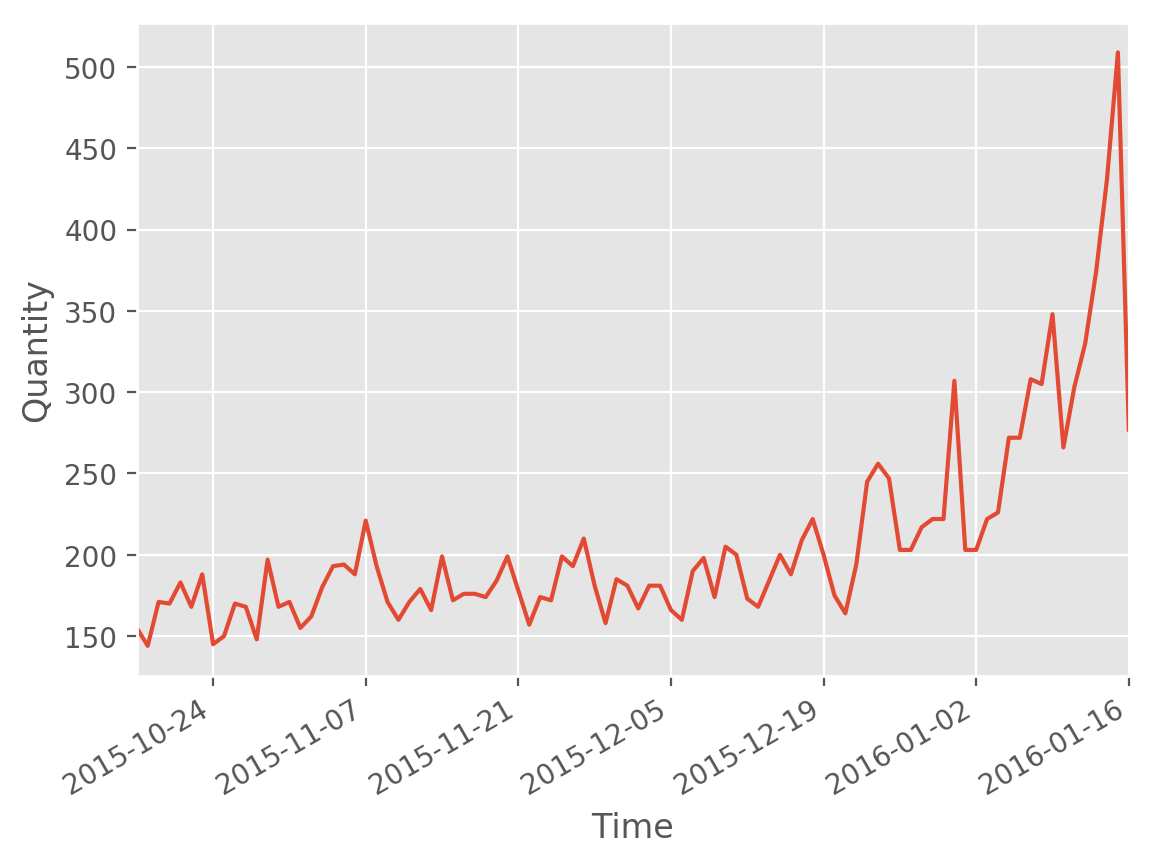
\includegraphics[width=\columnwidth]{quantity_time_graph}
\caption{貼文數量對時間的關係圖}
\label{f1}
\end{figure}

\begin{figure}[!htbp]
\centering
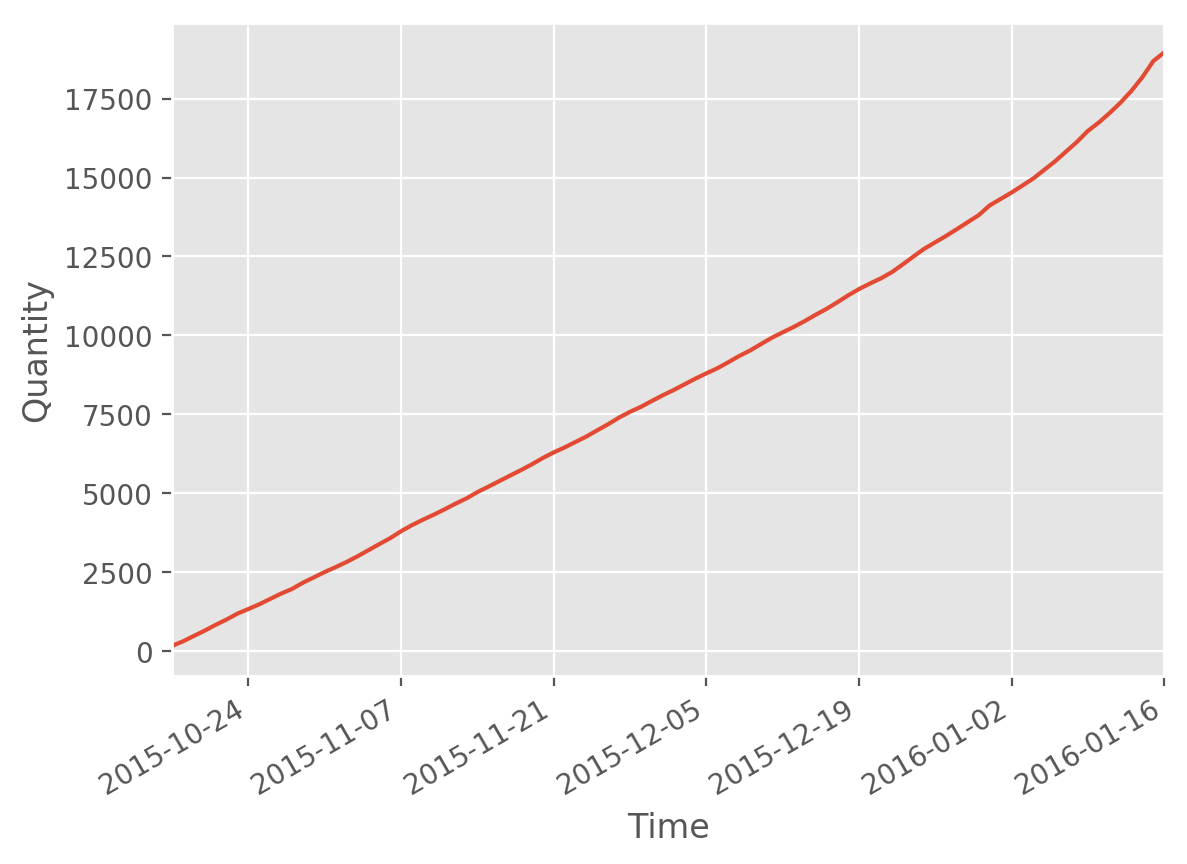
\includegraphics[width=\columnwidth]{quantity_time_cumulative_graph}
\caption{累計貼文數量對時間的關係圖}
\label{f2}
\end{figure}

接下來,表 \ref{t1} 列出了各政黨/侯選人/意見領袖的貼文數量,並依貼文數量遞減排序。%
發佈最多貼文的粉絲專頁是「柯建銘」,其貼文佔了全部貼文的 2.56\%。%
此次選舉的三位總統候選人也都有相當高的貼文數。%
此外,有幾個粉絲專頁在競選期間沒有發佈任何貼文(也可能是有發佈貼文但事後又被刪除,%
或因故無法透過 Facebook Graph API 存取),因此並未出現在表上。%

\onecolumn

\begin{longtable}[c]{@{}lcc@{}}
\caption{各政黨/侯選人/意見領袖的貼文數量}
\label{t1}\\
\toprule
粉絲專頁名稱 & 貼文數量 & 百分比 \\* \midrule
\endfirsthead
\toprule
粉絲專頁名稱 & 貼文數量 & 百分比 \\* \midrule
\endhead
%
\bottomrule
\endfoot
%
\endlastfoot
%
柯建銘 & 485 & 2.56\% \\
Taiwan Fugue & 361 & 1.90\% \\
台灣新力量/羅致政粉絲團 & 337 & 1.78\% \\
宋楚瑜找朋友 & 334 & 1.76\% \\
反馬英九聯盟 & 330 & 1.74\% \\
林昶佐 Freddy Lim & 320 & 1.69\% \\
基進黨(基進側翼) & 319 & 1.68\% \\
BillyPan 潘建志醫師 & 306 & 1.61\% \\
宋楚瑜 & 301 & 1.59\% \\
綠黨 & 297 & 1.57\% \\
民主進步黨 & 293 & 1.54\% \\
鄭永金後援會 & 282 & 1.49\% \\
我是台灣人 (I am Taiwanese) & 281 & 1.48\% \\
江啟臣服務讚 & 262 & 1.38\% \\
鄭正鈐 & 259 & 1.37\% \\
打馬悍將粉絲團 & 255 & 1.34\% \\
中國國民黨 KMT & 254 & 1.34\% \\
徐欣瑩 & 250 & 1.32\% \\
馬躍.比吼 Mayaw Biho & 250 & 1.32\% \\
蔡英文 Tsai Ing-wen & 249 & 1.31\% \\
大安推范雲 & 246 & 1.30\% \\
公民1985行動聯盟 & 246 & 1.30\% \\
洪慈庸 & 242 & 1.28\% \\
馬英九下台下台粉絲團 & 241 & 1.27\% \\
挺馬英九聯盟 & 231 & 1.22\% \\
呂欣潔 Jennifer Lu & 230 & 1.21\% \\
王如玄 & 220 & 1.16\% \\
黃韻涵粉絲頁 & 219 & 1.15\% \\
社會民主黨 & 219 & 1.15\% \\
朱立倫 & 214 & 1.13\% \\
吳秉叡 & 199 & 1.05\% \\
段宜康 & 198 & 1.04\% \\
鄭弘儀 & 197 & 1.04\% \\
陳其邁 Chen Chi-Mai & 195 & 1.03\% \\
公民廟口-立委在做天在看 & 194 & 1.02\% \\
時代力量 New Power Party & 194 & 1.02\% \\
沃草 Watchout & 193 & 1.02\% \\
林佳龍 & 190 & 1.00\% \\
鍾佳濱 & 190 & 1.00\% \\
苗博雅 MiaoPoya & 189 & 1.00\% \\
徐永明 & 186 & 0.98\% \\
趙正宇 & 185 & 0.98\% \\
小聖蚊的治國日記 & 184 & 0.97\% \\
魏明谷 & 183 & 0.96\% \\
鄭文燦 & 182 & 0.96\% \\
好立委 楊瓊瓔 & 179 & 0.94\% \\
張花冠(小花)縣長 & 177 & 0.93\% \\
潘孟安 & 176 & 0.93\% \\
管碧玲 (kuanbiling) & 175 & 0.92\% \\
白色正義聯盟 & 175 & 0.92\% \\
蔡正元 & 175 & 0.92\% \\
我是台灣人.台灣是咱的國家 & 175 & 0.92\% \\
立法委員 黃國昌 & 170 & 0.90\% \\
祭止兀 & 169 & 0.89\% \\
樹黨 & 166 & 0.88\% \\
不禮貌鄉民團 & 166 & 0.88\% \\
批踢踢實業坊(Ptt.cc) & 155 & 0.82\% \\
楊實秋 & 154 & 0.81\% \\
幸福好粽 鍾易仲 & 150 & 0.79\% \\
我是新竹人 & 148 & 0.78\% \\
Appendectomy Project 割闌尾計畫 & 145 & 0.76\% \\
王金平 & 142 & 0.75\% \\
特急件小周的人渣文本 & 142 & 0.75\% \\
王丹网站 Wang Dan's Page & 138 & 0.73\% \\
民國黨 & 138 & 0.73\% \\
李進勇 & 137 & 0.72\% \\
王定宇 & 136 & 0.72\% \\
徐耀昌加油讚 & 131 & 0.69\% \\
賴清德 & 130 & 0.69\% \\
陳菊 (花媽) 市長 & 129 & 0.68\% \\
我是中壢人 & 124 & 0.65\% \\
林智堅 & 121 & 0.64\% \\
游錫堃 & 120 & 0.63\% \\
徐巧芯 & 119 & 0.63\% \\
邱鏡淳 & 116 & 0.61\% \\
醫勞盟 & 115 & 0.61\% \\
社會民主連線 & 112 & 0.59\% \\
綠黨桃竹苗支黨部 & 110 & 0.58\% \\
台灣勞工陣線協會 & 109 & 0.57\% \\
蔣萬安 & 109 & 0.57\% \\
費鴻泰(阿力克司) & 109 & 0.57\% \\
謝長廷 & 107 & 0.56\% \\
拷秋勤 Kou Chou Ching & 107 & 0.56\% \\
吳宜臻 & 105 & 0.55\% \\
洪秀柱 & 105 & 0.55\% \\
蔡錦隆加油讚 & 103 & 0.54\% \\
劉文雄(Liu Wen Hsiung) & 101 & 0.53\% \\
林聰賢 & 98 & 0.52\% \\
嘉義市長涂醒哲 & 97 & 0.51\% \\
民主鬥陣 Democracy Tautin & 96 & 0.51\% \\
nagee & 96 & 0.51\% \\
島國前進 Taiwan March & 91 & 0.48\% \\
柯文哲 & 89 & 0.47\% \\
馮光遠 & 89 & 0.47\% \\
捍衛苗栗青年聯盟 & 88 & 0.46\% \\
葉宜津 & 84 & 0.44\% \\
張承中 & 83 & 0.44\% \\
張麗善粉絲團 & 80 & 0.42\% \\
法操FOLLAW & 77 & 0.41\% \\
民間司法改革基金會 & 74 & 0.39\% \\
林志嘉 & 70 & 0.37\% \\
蘇貞昌 & 66 & 0.35\% \\
全國廢核行動平台 & 64 & 0.34\% \\
國民黨青年團 & 63 & 0.33\% \\
反黑箱服貿協議 & 57 & 0.30\% \\
鍾年晃 & 51 & 0.27\% \\
鄉民實業坊 & 50 & 0.26\% \\
馬英九 & 49 & 0.26\% \\
周芷萱 斬父權獨立劍 老娘就是反骨! & 49 & 0.26\% \\
藍白拖的逆襲 & 43 & 0.23\% \\
林右昌UChange & 42 & 0.22\% \\
台灣農村陣線 & 42 & 0.22\% \\
施明德 & 34 & 0.18\% \\
台北市議員徐弘庭 & 30 & 0.16\% \\
台北。生生不息。王閔生 & 29 & 0.15\% \\
反黑箱課綱行動聯盟 & 18 & 0.09\% \\
吳志剛 & 17 & 0.09\% \\
黑色島國青年陣線 & 16 & 0.08\% \\
{[}我是學生,我反旺中{]} 反媒體巨獸青年聯盟 & 15 & 0.08\% \\
連勝文 & 15 & 0.08\% \\
反洗腦課綱學生陣線 & 13 & 0.07\% \\
無限期支持警察 & 12 & 0.06\% \\
周守訓 & 6 & 0.03\% \\
方仰寧加油 & 5 & 0.03\% \\
民進黨台灣民主學院 & 3 & 0.02\% \\
顧立雄 & 2 & 0.01\% \\
Tumorectomy Project 割腫瘤計畫 & 1 & 0.01\% \\
台大法律學生挺318 & 1 & 0.01\% \\* \bottomrule
\end{longtable}

\begin{longtable}[c]{@{}L{2.45cm}L{1.1cm}L{1.1cm}L{1.1cm}L{1.1cm}L{1.1cm}L{1.1cm}L{1.1cm}L{1.1cm}L{1.1cm}L{1.1cm}@{}}
\caption{關鍵字擷取,依作者劃分}
\label{t2}\\
\toprule
粉絲專頁名稱 & \#1 & \#2 & \#3 & \#4 & \#5 & \#6 & \#7 & \#8 & \#9 & \#10 \\* \midrule
\endfirsthead
\toprule
粉絲專頁名稱 & \#1 & \#2 & \#3 & \#4 & \#5 & \#6 & \#7 & \#8 & \#9 & \#10 \\* \midrule
\endhead
%
\bottomrule
\endfoot
%
\endlastfoot
%
朱立倫 & 台灣 & 新 & 孩子 & 支持 & 推動 & 政策 & 國民黨 & 北市 & 經濟 & 中 \\
大安推范雲 & 范雲 & 台灣 & 政治 & 中 & 感謝 & 朋友 & 支持 & 新 & 立委 & 大安 \\
王丹网站 Wang Dan's Page & 中國 & 中 & 大學 & 朋友 & 運動 & 台灣 & 件 & 國家 & 臺灣 & 老師 \\
國民黨青年團 & 青年 & 台灣 & 活動 & 力量 & 總統 & 朱立倫 & 主席 & 青年團 & 報名 & 時間 \\
呂欣潔 Jennifer Lu & 政治 & 欣潔 & 台灣 & 中 & 呂欣潔 & 朋友 & 希望 & 支持 & 新 & 照顧 \\
管碧玲 (kuanbiling) & 管媽 & 市長 & 台灣 & 高雄 & 朋友 & 旗津 & 中 & 總部 & 市民 & 第一 \\
段宜康 & 朱立倫 & 國民黨 & 王如玄 & 台灣 & 新 & 公司 & 買 & 委員 & 兩 & 候選人 \\
鄉民實業坊 & 黑子 & 種 & 書 & 中 & 現場 & 文章 & 真的 & 幫 & Chenglap & 11 \\
我是台灣人 (I am Taiwanese) & 台灣 & 綠黨 & 聯盟 & 國民黨 & 政黨 & 中 & 政治 & 立委 & 支持 & 新 \\
林智堅 & 新竹市 & 新竹 & 市民 & 服務 & 中 & 城市 & 客家 & 朋友 & 台灣 & 座 \\
BillyPan 潘建志醫師 & 醫師 & 台灣 & 潘建志 & 潘 & 潘醫師 & 中 & 支持 & 朋友 & 號 & 感謝 \\
蔡錦隆加油讚 & 蔡錦隆 & 錦隆 & 台灣 & 總部 & 競選 & 台中 & 鄉親 & 今日 & 立委 & 舉辦 \\
馬英九 & 臺灣 & 中 & 政府 & 兩 & 阿嬤 & 我國 & 兩岸 & 中華民國 & 國際 & 孩子 \\
醫勞盟 & 醫師 & 醫療 & 健保 & 醫院 & 元 & 病人 & 醫勞盟 & 人員 & 月 & 健保署 \\
陳其邁 Chen Chi-Mai & 國民黨 & 元 & 中 & 台灣 & 食品 & 總統 & 民進黨 & 朱立倫 & 抹黑 & 約 \\
中國國民黨 KMT & 台灣 & 朱立倫 & 國民黨 & 未來 & 經濟 & 兩岸 & 政策 & 立委 & 主席 & 國家 \\
徐欣瑩 & 台灣 & 欣瑩 & 徐欣瑩 & 民國黨 & 民眾 & 人民 & 中 & 政治 & 主席 & 鄉親 \\
全國廢核行動平台 & 能源 & 核 & 台電 & 核電 & 核電廠 & 政府 & 核災 & 台灣 & 中 & 核四 \\
柯文哲 & 台北 & 政府 & 市民 & 市府 & 中 & 台北市 & 臺北市 & 工作 & 台灣 & 臺北 \\
白色正義聯盟 & 台灣 & 支持 & 白盟 & 民進黨 & 兩岸 & 國民黨 & 小編 & 馬 & 中 & 總統 \\
台灣勞工陣線協會 & 勞工 & 台灣 & 勞動 & 工作 & 政府 & 工會 & 中國 & 勞陣 & 元 & 經濟 \\
謝長廷 & 國民黨 & 台灣 & 候選人 & 民進黨 & 總統 & 立委 & 英文 & 蔡 & 兩 & 曾 \\
柯建銘 & 柯建銘 & 新竹 & 國會 & 新竹市 & 台灣 & 國民黨 & 民進黨 & 柯 & 改革 & 總召 \\
法操FOLLAW & 檢察官 & 大法客 & 證據 & 法官 & 起訴 & 新 & 案 & 頂 & 司法 & Q \\
王定宇 & 台南 & 定宇 & 永康 & 國民黨 & 點 & 仁德 & 中 & 來到 & 台灣 & 參加 \\
鄭永金後援會 & 新竹 & 鄭永金 & 台灣 & 新竹縣 & 鄉親 & 蔡英文 & 支持 & 客家 & 活動 & 感謝 \\
黃韻涵粉絲頁 & 韻涵 & 活動 & 岡山 & 高雄 & 希望 & 中 & 支持 & 感謝 & 鄉親 & 一同 \\
小聖蚊的治國日記 & 國民黨 & 台灣 & 朱立倫 & 話 & 馬英九 & 支持 & 新聞 & 民進黨 & 蛆 & 食安 \\
民主進步黨 & 全文 & 台灣 & 蔡英文 & 號 & 民進黨 & 產業 & 新 & 立委 & 國民黨 & 改革 \\
周芷萱 斬父權獨立劍 老娘就是反骨! & 台灣 & 性 & 中 & 種 & 社會 & 女性 & 性別 & 女人 & 工作 & 老娘 \\
賴清德 & 台南 & 台灣 & 朋友 & 文化 & 市民 & 中 & 新 & 市府 & 台南市 & 感謝 \\
Taiwan Fugue & 國民黨 & 朱立倫 & 台灣 & 馬英九 & 立委 & 新 & 中國 & 總統 & 王如玄 & 中 \\
林佳龍 & 台中 & 市府 & 台灣 & 台中市 & 中 & 希望 & 元 & 市民 & 未來 & 活動 \\
公民廟口-立委在做天在看 & 台灣 & 立委 & 真的 & 種 & 中國 & 想 & 國民黨 & 國會 & 政府 & 中 \\
吳秉叡 & 新莊 & 台灣 & 秉 & 鄉親 & 大秉 & 新 & 小英 & 立委 & 秉叡 & 中 \\
張承中 & 政府 & 兩 & 想 & 民調 & 朋友 & 11 & 整合 & 企業 & 公益 & 希望 \\
幸福好粽 鍾易仲 & 易仲 & 鄉親 & 美濃 & 邱議瑩 & 立委 & 高雄市 & 高雄 & 台灣 & 水 & 鍾易仲 \\
鄭弘儀 & 寶島 & 台灣 & 大哥 & 世界 & 節目 & 鄭 & 中國 & 聯播網 & 馬英九 & 管理員 \\
趙正宇 & 正宇 & 桃園 & 活動 & 趙正宇 & 八德 & 改變 & 支持 & 八德區 & 力量 & 新 \\
我是中壢人 & 中壢 & 桃園 & 仲介 & 台灣 & 學生 & 點 & 學校 & 中 & 時間 & 教學 \\
王金平 & 國會 & 改革 & 台灣 & 立委 & 國民黨 & 委員 & 立法院 & 支持 & 民進黨 & 人民 \\
黑色島國青年陣線 & 馬英九 & 人民 & 台灣 & 總統 & 中國 & 馬習會 & 政府 & 中 & 透過 & 國民黨 \\
邱鏡淳 & 新竹縣 & 台灣 & 鏡淳 & 活動 & 新竹 & 民眾 & 竹東 & 縣府 & 日 & 中 \\
台灣新力量/羅致政粉絲團 & 板橋 & 台灣 & 羅致政 & 新 & 致政 & 選舉 & 蔡英文 & 朋友 & 中 & 活動 \\
蔡正元 & 蔡英文 & 台灣 & 政治 & 大陸 & 中國 & 美國 & 兩岸 & 種 & 中 & 民進黨 \\
林右昌UChange & 基隆 & 台灣 & 基隆市 & 市府 & 昌 & 中心 & 城市 & 右 & 市民 & 活動 \\
鄭正鈐 & 正鈐 & 新竹 & 新竹市 & 鄭正鈐 & 朋友 & 總部 & 柯建銘 & 選舉 & 中 & 台灣 \\
葉宜津 & 台灣 & 土地 & 民進黨 & 國家 & 豬 & 感謝 & ㄧ & 喜樹 & 人民 & 支持 \\
江啟臣服務讚 & 啟臣 & 豐原 & 鄉親 & 新 & 新社 & 東勢 & 中 & 民眾 & 活動 & 服務 \\
好立委 楊瓊瓔 & 瓊瓔 & 鄉親 & 台中 & 后里 & 楊瓊瓔 & 台灣 & 支持 & 活動 & 孩子 & 潭子 \\
鍾佳濱 & 屏東 & 台灣 & 佳濱 & 未來 & 縣長 & 期待 & 選舉 & 裡 & 政策 & 新 \\
台灣農村陣線 & 土地 & 台灣 & 政府 & 農業 & 農村 & 農民 & 徵收 & 中 & 糧食 & 小農 \\
台北市議員徐弘庭 & 中 & 台灣 & 家 & 市場 & 證所稅 & 好朋友 & 點 & 協會 & 台北 & 委員 \\
綠黨桃竹苗支黨部 & 台灣 & 綠黨 & 聯盟 & 政治 & 社會民主黨 & 社會 & 環境 & 兩 & 財團 & 人民 \\
周守訓 & 第一 & 喜樂 & 剩 & 2016 & 聖誕餅 & 祝福 & 老板 & 酷酷 & 盤子 & 永遠 \\
陳菊 (花媽) 市長 & 高雄 & 台灣 & 中 & 城市 & 朋友 & 市民 & 活動 & 未來 & 文化 & 人民 \\
挺馬英九聯盟 & 台灣 & 總統 & 民進黨 & 蔡英文 & 中華民國 & 種 & 馬 & 兩岸 & 蔡 & 政治 \\
沃草 Watchout & 立委 & 立法院 & 候選人 & 中 & 台灣 & 阿草 & 立院 & 臺灣 & 中國 & 國民黨 \\
張花冠(小花)縣長 & 嘉義 & 嘉義縣 & 文化 & 社區 & 台灣 & 故宮 & 阿里山 & 活動 & 中 & 內 \\
Appendectomy Project 割闌尾計畫 & 落選 & 闌尾 & 立委 & 罷免 & 割 & 吳育昇 & 委員 & 台灣 & 運動 & 中 \\
批踢踢實業坊(Ptt.cc) & 鄉民 & 原 & 世界 & 投票 & 真的 & 台灣 & 談 & 專業 & 媒體 & 笑 \\
林聰賢 & 宜蘭 & 台灣 & 中 & 縣府 & 宜蘭縣 & 朋友 & 新 & 民眾 & 同仁 & 種 \\
反馬英九聯盟 & 國民黨 & 朱立倫 & 馬英九 & 王如玄 & 立委 & 台灣 & 新 & 政府 & 軍宅 & 中國 \\
游錫堃 & 台灣 & 總統 & 小英 & 新 & 中 & 國民黨 & 北市 & 朱立倫 & 未 & 民進黨 \\
我是台灣人.台灣是咱的國家 & 台灣 & 國民黨 & 台灣人 & 中國 & 民進黨 & 中 & 總統 & 國會 & 選舉 & 朱立倫 \\
馮光遠 & 台灣 & 國民黨 & 片名 & 中 & 馬英九 & 裡 & 眉批 & 朱立倫 & 事 & 吳育昇 \\
綠黨 & 台灣 & 綠黨 & 中 & 聯盟 & 政治 & 勞工 & 社會民主黨 & 綠社盟 & 環境 & 政府 \\
民主鬥陣 Democracy Tautin & 台灣 & 中國 & 中 & 貨貿 & 政府 & 人民 & 貿易 & 民主 & 產業 & 談判 \\
方仰寧加油 & 街頭 & 藝人 & 日 & 國 & 國際 & 2015 & 路 & 海安 & 陳國 & 2000萬 \\
劉文雄(Liu Wen Hsiung) & 基隆 & 台灣 & 國家 & 民眾 & 政府 & 老百姓 & 財團 & 事 & 花 & 市長 \\
顧立雄 & 偏鄉 & 高 & 律師 & 募款 & 平台 & 牆 & 20 & 餐會 & 司改會 & 教 \\
公民1985行動聯盟 & 台灣 & 社會 & 立委 & 種 & 政府 & 真的 & 想 & 國會 & 中 & 兵團 \\
潘孟安 & 屏東 & 台灣 & 中 & 新 & 種 & 縣府 & 活動 & 推動 & 屏東縣 & 文化 \\
無限期支持警察 & 警察 & 執法 & 支持 & 員警 & 單位 & 警察局 & 判決 & 同仁 & 人員 & 捍衛 \\
樹黨 & 樹黨 & 候選人 & 台灣 & 立委 & 樹 & 新 & 號 & 黨 & 樹木 & 政黨 \\
我是新竹人 & 新竹 & 台灣 & 新竹市 & 綠黨 & 中 & 時間 & 民進黨 & 國民黨 & 元 & 候選人 \\
{[}我是學生,我反旺中{]} 反媒體巨獸青年聯盟 & 台灣 & 活動 & 月 & NCC & 新 & 頂 & 關係法 & 11 & 公民 & 份 \\
鄭文燦 & 桃園 & 市府 & 台灣 & 活動 & 桃園市 & 市民 & 計畫 & 包括 & 中心 & 文化 \\
基進黨(基進側翼) & 台灣 & 中國 & 中 & 基進 & 政治 & 側翼 & 國民黨 & 新 & 社會 & 陳奕齊 \\
nagee & 台灣 & 中國 & 國民黨 & 政府 & 種 & 國家 & 台灣人 & 人民 & 馬英九 & 中 \\
民進黨台灣民主學院 & 客家 & 大學 & 青年 & 報名 & 交通 & 電話 & 當選 & 1月 & 參加 & 民主 \\
林昶佐 Freddy Lim & 林昶佐 & 台灣 & 中 & 支持 & 昶佐 & 林郁方 & 閃靈 & 立委 & 政治 & 萬華 \\
楊實秋 & 楊實秋 & 國民黨 & 台灣 & 選舉 & 政治 & 支持 & 總統 & 中 & 未來 & 名 \\
徐耀昌加油讚 & 徐耀昌 & 苗栗 & 縣長 & 縣府 & 舉辦 & 苗栗縣 & 社區 & 活動 & 推動 & 文化 \\
吳宜臻 & 臻 & 宜 & 苗栗 & 鄉親 & 選舉 & 台灣 & 希望 & 立委 & 小英 & 市長 \\
徐巧芯 & 民進黨 & 蔡英文 & 總統 & 國民黨 & 主席 & 辯論 & 王如玄 & 民眾 & 支持 & 兩岸 \\
反黑箱課綱行動聯盟 & 課綱 & 教育部 & 學生 & 教育 & 政治 & 微調 & 台灣 & 政策 & 反 & 會議 \\
祭止兀 & 支持 & 台灣 & 總統 & 止兀 & 兩 & 票 & 愛 & 選 & 太 & 柯 \\
立法委員 黃國昌 & 新 & 台灣 & 汐止 & 國昌 & 瑞芳 & 鄉親 & 幸福 & 政治 & 北市 & 社會 \\
鍾年晃 & 台灣 & 國民黨 & 蔡英文 & 土地 & 中國 & 民進黨 & 共識 & 坪 & 議題 & 馬英九 \\
蘇貞昌 & 新 & 台灣 & 鄉親 & 立委 & 北市 & 選區 & 國會 & 蔡英文 & 總統 & 參加 \\
李進勇 & 雲林 & 雲林縣 & 縣府 & 活動 & 元 & 台灣 & 服務 & 補助 & 北港 & 咖啡 \\
蔡英文 Tsai Ing-wen & 台灣 & 人民 & 中 & 政府 & 社會 & 新 & 國家 & 改革 & 民進黨 & 產業 \\
捍衛苗栗青年聯盟 & 台灣 & 中國 & 國民黨 & 中 & 立委 & 計畫 & 政府 & 種 & 國家 & 無 \\
張麗善粉絲團 & 雲林 & 執行長 & 台灣 & 麗善 & 雲嘉南 & 鎔麒 & 中心 & 服務 & 立委 & 行政院 \\
馬英九下台下台粉絲團 & 國民黨 & 馬英九 & 總統 & 台灣 & 朱立倫 & 新 & 鄉民 & 兩 & 馬 & 元 \\
宋楚瑜找朋友 & 台灣 & 政府 & 主席 & 宋楚瑜 & 人民 & 總統 & 宋 & 小宋 & 兩 & 國家 \\
反黑箱服貿協議 & 台灣 & 中國 & 政府 & 民主 & 貨貿 & 中 & 馬 & 地區 & 談判 & 大陸 \\
不禮貌鄉民團 & 國民黨 & 台灣 & 中國 & 票 & 種 & 政府 & 民進黨 & 裡 & 想 & 選舉 \\
馬躍.比吼 Mayaw Biho & 馬躍 & 原住民 & 部落 & 文化 & 族人 & 中 & 土地 & 原住民族 & 台灣 & 朋友 \\
拷秋勤 Kou Chou Ching & 新聞 & 台灣 & 國民黨 & 中國 & 中 & KMT & 新 & 臺灣 & 朱立倫 & 689 \\
島國前進 Taiwan March & 台灣 & 人民 & 連署 & 落選 & 立委 & 00 & 島國 & 運動 & 政府 & 公投 \\
社會民主連線 & 政府 & 香港 & 社會 & 梁振英 & 名 & 全民 & 社民 & 市民 & 亦 & 立法會 \\
魏明谷 & 彰化 & 彰化縣 & 台灣 & 活動 & 縣府 & 中 & 政府 & 民眾 & 高鐵 & 國 \\
嘉義市長涂醒哲 & 嘉義市 & 嘉義 & 市府 & 市民 & 文化 & 新 & 台灣 & 活動 & 未來 & 健康 \\
施明德 & 台灣 & 中 & 人民 & 烏魚 & 總統 & 中華民國 & 國民黨 & 國際 & 國軍 & 國家 \\
Tumorectomy Project 割腫瘤計畫 & None & None & None & None & None & None & None & None & None & None \\
吳志剛 & 委員 & 門診 & 整合 & 病人 & 市長 & 希望 & 萬華區 & 剛 & 參加 & 物資 \\
徐永明 & 力量 & 時代 & 台灣 & 國會 & 人民 & 新 & 2016 & 挺 & 政治 & 國民黨 \\
打馬悍將粉絲團 & 國民黨 & 朱立倫 & 台灣 & 真的 & 中國 & 版主 & 新聞 & 馬英九 & 投票 & 連結 \\
連勝文 & 朋友 & 創業 & 創意 & 希望 & 兩岸 & 社區 & 台灣 & 中 & 參加 & 活動 \\
林志嘉 & 台灣 & 台聯 & 中國 & 國民黨 & 中 & 人民 & 總統 & 立法院 & 政府 & 馬英九 \\
台北。生生不息。王閔生 & 蔡英文 & 兒童 & 台北市 & 服務 & 家庭 & 主席 & 元 & 台灣 & 同志 & 市府 \\
反洗腦課綱學生陣線 & 課綱 & 立委 & 委員 & 學生 & 微調 & 民進黨 & 歷史 & 點 & 鄭麗君 & 台聯 \\
台大法律學生挺318 & None & None & None & None & None & None & None & None & None & None \\
民國黨 & 台灣 & 民國黨 & 政府 & 徐欣瑩 & 人民 & 政策 & 國家 & 經濟 & 主席 & 希望 \\
社會民主黨 & 台灣 & 社會民主黨 & 立委 & 聯盟 & 中 & 綠社盟 & 勞工 & 政治 & 總統 & 綠黨 \\
洪秀柱 & 國家 & 黨 & 中 & 兩岸 & 柱柱姐 & 支持 & 國民黨 & 人民 & 希望 & 政治 \\
蔣萬安 & 萬安 & 朋友 & 民眾 & 活動 & 鄉親 & 臺灣 & 未來 & 希望 & 服務 & 長輩 \\
苗博雅 MiaoPoya & 阿苗 & 政治 & 台灣 & 立委 & 中 & 國會 & 新 & 馬習會 & 社會 & 支持 \\
洪慈庸 & 慈庸 & 台灣 & 青年 & 中 & 政治 & 后里 & 社會 & 朋友 & 人民 & 大雅 \\
王如玄 & 台灣 & 王如玄 & OneTaiwan & 朋友 & 婦女 & 中 & 玄 & 勞工 & 手 & 社會 \\
時代力量 New Power Party & 台灣 & 力量 & 時代 & 人民 & 中 & 政府 & 國會 & 中國 & 政治 & 國民黨 \\
費鴻泰(阿力克司) & 鴻泰 & 市場 & 服務 & 朋友 & 費鴻泰 & 號 & 鄉親 & 活動 & 感謝 & 費 \\
藍白拖的逆襲 & 民進黨 & 台灣 & 傳送門 & 大陸 & 蔡英文 & 小編 & 中 & 中國 & 總統 & 國民黨 \\
民間司法改革基金會 & 律師 & 司法 & 法官 & 檢察官 & 台灣 & 案件 & 人民 & 法院 & 法律 & 判決 \\
宋楚瑜 & 台灣 & 政府 & 宋楚瑜 & 小宋 & 主席 & 人民 & 總統 & — & 國家 & 宋 \\
特急件小周的人渣文本 & 國民黨 & 種 & 中 & 想 & 台灣 & 選舉 & 新 & 講 & 政治 & 朱立倫 \\* \bottomrule
\end{longtable}

\twocolumn

\subsection*{關鍵字擷取(keyword extraction)}

在這裡輸入文字。%

\subsection*{情感分析(sentiment analysis)}

結果見表。%

\subsection*{社會互動(social interaction)}

結果見圖。%

\section*{五、結論}

在這裡輸入文字。%

\addtolength{\textheight}{-12cm}  % This command serves to balance the column lengths
                                  % on the last page of the document manually. It shortens
                                  % the textheight of the last page by a suitable amount.
                                  % This command does not take effect until the next page
                                  % so it should come on the page before the last. Make
                                  % sure that you do not shorten the textheight too much.

%%%%%%%%%%%%%%%%%%%%%%%%%%%%%%%%%%%%%%%%%%%%%%%%%%%%%%%%%%%%%%%%%%%%%%%%%%%%%%%%

\section*{附錄}

在這裡輸入文字。%

\section*{誌謝}

首先,我要感謝我的指導教授孫春在教授,對我的研究給予了許多寶貴的建議。%
另外,我要感謝中央研究院資訊科學研究所中文詞知識庫小組,提供中文斷詞線上服務。%
有您們的協助,這份研究才得以順利完成。%

%%%%%%%%%%%%%%%%%%%%%%%%%%%%%%%%%%%%%%%%%%%%%%%%%%%%%%%%%%%%%%%%%%%%%%%%%%%%%%%%

\bibliographystyle{ieeetr}
\bibliography{citation}

\end{CJK}
\end{document}
